\documentclass[hidelinks,a4paper,10pt, nofootinbib]{article}
\usepackage[width=15.5cm, left=3cm, top=2.5cm, right=2cm, left=2cm, height= 24.5cm]{geometry}
\usepackage[spanish]{babel}
\usepackage[utf8]{inputenc}
\usepackage[T1]{fontenc}
\usepackage{xspace}
\usepackage{xargs}
\usepackage{fancyhdr}
\usepackage{lastpage}
\usepackage{caratulaMetNum}
\usepackage[bottom]{footmisc}
\usepackage{amssymb}
\usepackage{amsmath}
\usepackage{algorithm}
\usepackage[noend]{algpseudocode}

\usepackage{graphicx}
\usepackage{sidecap}
\usepackage{wrapfig}
\usepackage{caption}


%%fancyhdr
\pagestyle{fancy}
\thispagestyle{fancy}
\addtolength{\headheight}{1pt}
\lhead{Organización del Computador II: TP2}
\rhead{$2º$ cuatrimestre de 2015}
\cfoot{\thepage\ / \pageref{LastPage}}
\renewcommand{\footrulewidth}{0.4pt}

%%caratula
\materia{Organización del Computador II}
\titulo{Trabajo Práctico Número 2}
\subtitulo{Con 15 $\theta$'s discretizo alto horno}
\grupo{Grupo: Tu me pixeleas}
\integrante{Costa, Manuel José Joaquín}{035/14}{manuc94@hotmail.com}
\integrante{Gatti, Mathias Nicolás}{477/14}{mathigatti@gmail.com}
\integrante{Pondal, Iván}{078/14}{ivan.pondal@gmail.com}


\begin{document}
\maketitle
\section{Introducción}
El objetivo de este trabajo fue estudiar e implementar en una aplicación real el
modelo de procesamiento SIMD (Single Instruction Multiple Data). Para esto se
nos encomendó la tarea de desarrollar en C y ASM (Intel64) dos filtros de
imágenes con los cuales debíamos por un lado analizar cómo competían las
implementaciones y por otro lado realizar un experimento adicional en base al
trabajo ya hecho con el fin de profundizar el estudio del mismo.

Los filtros en cuestión fueron \textit{Diferencia de Imágenes} y \textit{Blur
Gaussiano}. El primero, dado dos imágenes del mismo tamaño, genera una imagen de salida
en escala de grises donde las partes similares o iguales entre las dos entradas
se verán oscuras o negras, mientras que las que difieran, aparecerán más
blancas. El segundo, dada una imagen, un coeficiente real $\sigma$ y un \textit{r}
entero, genera una imágen desenfocada en base a los parámetros de entrada.

Para \textit{Diferencia de Imágenes}, se realizó el estudio de rendimiento entre
la implementación en C y la de ASM utilizando SIMD. En lo que respecta
\textit{Blur Gaussiano}, también se hizo la prueba de performance entre
implementaciones con la diferencia de que en C realizamos dos códigos distintos
donde uno presenta una optimización vinculada con la forma en la que calcula
la convolución necesaria para el efecto. A su vez, decidimos experimentar con el
balance entre performance y precisión del filtro, para lo cual desarrollamos
una segunda implementación en ASM con la que buscamos procesar más datos en
simultáneo sacrificando precisión en las cuentas.

\newpage

\section{Desarrollo}
\subsection{Diferencia de imagenes}

\subsubsection{Explicación del código en assembler}
El código sigue el siguiente esquema:
\begin{enumerate}
	\item Cálculo del total de píxeles de la imagen.
	\item Ciclo en el que procesamos de a cuatro píxeles por iteración:
	\begin{enumerate}
		\item Cargamos los píxeles y desempaquetamos las componentes de bytes a words, pues vamos a restar enteros de un byte sin signo (entre 0 y 255), lo que puede dar resultados entre -255 y 255.
		\item Realizamos las restas y tomamos valor absoluto de los resultados.
		\item Empaquetamos nuevamente a byte las componentes (que ahora son todas positivas).
		\item Calculamos la componente máxima de cada vector (sin incluir la transparencia), que queda guardada en la componente \emph{r}.
		\item Seteamos todas las componentes de cada vector con el valor de su norma infinito, salvo la transparencia que ponemos en 255 siempre. 
		\item Avanzamos los punteros.
	\end{enumerate}
\end{enumerate}

Pasamos a detallar un poco más cada punto.




\subsection{Blur Gaussiano}
\label{sec:blur_imp}

\subsubsection{Descripción del filtro}
\label{sec:blur_desc}

El filtro \textit{Blur Gaussiano}, produce un desenfoque en la imagen original
en base a un coeficiente $\sigma$ y \textit{r} entero. Estas variables son
parámetros que afectan por un lado, la dispersión o varianza de la distribución
normal de Gauss, y por el otro, la discretización de la misma. El uso de la
función de densidad de la distribución normal es clave para el resultado del
efecto ya que el mismo es el resultado de realizar un promedio ponderado de
los vecinos de cada pixel, tomando como pesos los valores discretizados de la
función.

Esto tiene una consecuencia directa sobre el resultado del filtro, y es que si
tomamos un $\sigma$ grande, implicando mayor dispersión, y utilizamos un
\textit{r} pequeño, veremos que la imagen producida se verá oscurecida (Figura \ref{fig:blur_s3_r3}), esto
se debe a que nuestra función de densidad integra a 1 cuando se recorren todos
sus valores, pero al discretizar, la suma no llega a 1, se está recortando gran
parte de la imagen de la función. Una posible solución es aumentar el radio,
obteniendo así más valores de la función y permitiendo que la suma vaya
aproximándose a 1 (Figura \ref{fig:blur_s3_r6}).

\begin{figure}[H]
	\centering
	\begin{minipage}{.3\textwidth}
		\centering
		
\includegraphics[width=\linewidth]{imgs/blur_original.jpg}
		\caption{Imagen original}
		\label{fig:blur_original}
	\end{minipage}\hfill
	\begin{minipage}{.3\textwidth}
		\centering
		
\includegraphics[width=\linewidth]{imgs/blur_s3_r3.jpg}
		\caption{Blur  $\sigma = 3, r = 3$}
		\label{fig:blur_s3_r3}
	\end{minipage}\hfill
	\begin{minipage}{.3\textwidth}
		\centering
		
\includegraphics[width=\linewidth]{imgs/blur_s3_r6.jpg}
		\caption{Blur $\sigma = 3, r = 6$}
		\label{fig:blur_s3_r6}
	\end{minipage}
\end{figure}


A continuación se describirán las dos implementaciones que se realizaron en ASM
para lo cual antes comentaremos los principales componentes que aparecen
en las mismas. Por un lado tenemos las imágenes de entrada y la de salida, donde
comienzan siendo idénticas, y a medida que avanza el algoritmo, la de destino va
modificándose hasta llegar al resultado final. Por otra parte está la matriz de
convolución. Esta es de gran importancia, ya que es la que contiene todos los
coeficientes discretizados de la función de Gauss, y será la que al aplicarse
sobre los vecinos del pixel a procesar nos generará el promedio ponderado.

\subsubsection{Implementación de control}

Aquí desarrollaremos en detalle sobre la primer implementación en ASM, la de
control, cuya característica principal es mediante SIMD procesar de a pixeles
enteros las operaciones necesarias.

A grandes rasgo lo que el código lo que hará es ir aplicando la matriz de convolución a los pixeles que
componen la imagen de izquierda a derecha, de abajo hacia
arriba en la imagen.

\begin{table}[H]
	\centering
	\begin{tabular}{|ccc|}
		\hline
		$\longrightarrow$ & $\longrightarrow$ & $\longrightarrow$ \\ \hline
		$\longrightarrow$ & $\longrightarrow$ & $\uparrow$ \\ \hline
		$\longrightarrow$ & $\longrightarrow$ & $\uparrow$ \\ \hline
		$\longrightarrow$ & $\longrightarrow$ & $\uparrow$ \\ \hline
		$\longrightarrow$ & $\longrightarrow$ & $\uparrow$ \\ \hline
	\end{tabular}
	\caption{Orden de procesamiento}
\end{table}

Nuestro estado inicial será ubicando la matriz de convolución en la esquina
inferior izquierda de la imagen para lo cual vamos a definir algunas variables.

\begin{equation*}
	\begin{aligned}[c]
		\underset{\begin{subarray}{c}
			0 \leq i < alto(I) \\
			0 \leq j < 4*ancho(I)
	\end{subarray}}{I_{ij}} = byte_{ij} \\
	\text{Matriz de imagen original}
	\end{aligned}
	\qquad
	\begin{aligned}[c]
		\underset{\begin{subarray}{c}
			0 \leq i < alto(D) \\
			0 \leq j < 4*ancho(D)
	\end{subarray}}{D_{ij}} = byte_{ij} \\
	\text{Matriz de Imagen destino}
	\end{aligned}
	\qquad
	\begin{aligned}[c]
		\underset{\begin{subarray}{c}
			0 \leq i < alto(K) \\
			0 \leq j < ancho(K)
	\end{subarray}}{K_{ij}} = float_{ij} \\
	\text{Matriz de convolución (kernel)}
	\end{aligned}
\end{equation*}

Por la forma en que cargamos la imagen a memoria, el puntero a la misma comienza
apuntando el primer pixel desde la izquierda en la última fila. Por lo tanto
vamos a decir que la esquina inferior izquierda es $I_{0,0}$ y la esquina
superior derecha $I_{alto(I)-1,4*ancho(I)-1}$.

Para comenzar en nuestro estado inicial queremos superponer $K$ en nuestra
esquina inferior, para lo cual nuestro puntero a la imagen pasará a apuntar a
$I_{2*r,0}$.

A continuación supondremos que la imagen está en escala de grises, por lo que
cada componente (menos el canal de transparencia que será siempre 0) valdrá lo
mismo para facilitar la explicación.

\newcolumntype{C}[1]{>{\centering\arraybackslash}m{#1}}

\begin{enumerate}
	\item Ponemos nuestro acumulador para el valor final en 0. Utilizaremos un
		registro XMM que llamaremos XMM$_A$ con 4 floats empaquetados.
		\begin{table}[H]
			\centering
			\begin{tabular}{|*{4}{C{64pt}|}}
				\hline
				A & R & G & B \\ \hline
				0 & 0 & 0 & 0 \\ \hline
				float 3 & float 2 & float 1 & float 0 \\ \hline
				\multicolumn{4}{|c|}{128 bits} \\ \hline
			\end{tabular}
			\caption{XMM$_A$}
		\end{table}
	\item Ahora cargaremos de $I_{2*r,0}$ un pixel (4 bytes) a otro XMM que
		llamaremos XMM$_I$ mediante \textbf{movd}. Es importante destacar que
		los pixeles en memoria estarán al revés (BGRA en lugar de ARGB).
		\begin{table}[H]
			\centering
			\begin{tabular}{|*{4}{C{64pt}|}}
				\hline
				$I_{2*r,0}$ & $I_{2*r,1}$ & $I_{2*r,2}$ & $I_{2*r,3}$ \\ \hline
				B & G & R & A \\ \hline
				42 & 42 & 42 & 0 \\ \hline
				\multicolumn{4}{|c|}{32 bits} \\ \hline
			\end{tabular}
			\caption{Pixel $I_{2*r,0}$}
		\end{table}

		\begin{table}[H]
			\centering
			\begin{tabular}{|*{16}{C{18pt}|}}
				\cline{13-16} \multicolumn{12}{c|}{} & A & R & G & B \\ \hline
				- & - & - & - & - & - & - & - &- & - & - & - & 0 & 42 & 42 & 42 \\ \hline
				byte 15 & \multicolumn{11}{c|}{$\dots$} & byte 3 & byte 2 & byte 1 & byte 0 \\ \hline
				\multicolumn{16}{|c|}{128 bits} \\ \hline
			\end{tabular}
			\caption{XMM$_I$}
		\end{table}
	\item Cargamos de $K_{0,0}$ sólo el primer coeficiente a otro XMM que llamaremos
		XMM$_K$ mediante \textbf{movd}.
		\begin{table}[H]
			\centering
			\begin{tabular}{|C{64pt}|}
				\hline
				$K_{0,0}$ \\ \hline
				0.42 \\ \hline
				32 bits \\ \hline
			\end{tabular}
			\caption{Coeficiente $K_{0,0}$}
		\end{table}

		\begin{table}[H]
			\centering
			\begin{tabular}{|*{4}{C{64pt}|}}
				\cline{4-4} \multicolumn{3}{c|}{} & $K_{0,0}$ \\ \hline
				- & - & - & 0.42 \\ \hline
				float 3 & float 2 & float 1 & float 0 \\ \hline
				\multicolumn{4}{|c|}{128 bits} \\ \hline
			\end{tabular}
			\caption{XMM$_K$}
		\end{table}
	\item Ahora queremos pasar nuestros 4 bytes en XMM$_I$ a 4 ints para luego
		poder convertirlos a float y operar con ellos. Para esto usamos
		\textbf{pshufb} con la siguiente máscara:

		\textit{DB 0, 128, 128, 128, 1, 128, 128, 128, 2, 128, 128, 128, 3, 128, 128, 128}

		\begin{table}[H]
			\centering
			\begin{tabular}{|*{16}{C{18pt}|}}
				\cline{13-16} \multicolumn{12}{c|}{} & A & R & G & B \\ \hline
				- & - & - & - & - & - & - & - &- & - & - & - & 0 & 42 & 42 & 42 \\ \hline
				\multicolumn{16}{|c|}{128 bits} \\ \hline
			\end{tabular}
			\caption{XMM$_I$ antes de ejecutar \textbf{pshufb}}
		\end{table}

		\begin{table}[H]
			\centering
			\begin{tabular}{|*{16}{C{18pt}|}}
				\hline
				\multicolumn{4}{|c|}{A} & \multicolumn{4}{c|}{R} & \multicolumn{4}{c|}{G} & \multicolumn{4}{c|}{B} \\ \hline
				0 & 0 & 0 & 0 & 0 & 0 & 0 & 42 & 0 & 0 & 0 & 42 & 0 & 0 & 0 & 42 \\ \hline
				\multicolumn{16}{|c|}{128 bits} \\ \hline
			\end{tabular}
			\caption{XMM$_I$ después de ejecutar \textbf{pshufb}}
		\end{table}

	\item Convierto los int de XMM$_I$ a float.
		\begin{table}[H]
			\centering
			\begin{tabular}{|*{4}{C{64pt}|}}
				\hline
				A & R & G & B \\ \hline
				0.0 & 42.0 & 42.0 & 42.0 \\ \hline
				float 3 & float 2 & float 1 & float 0 \\ \hline
				\multicolumn{4}{|c|}{128 bits} \\ \hline
			\end{tabular}
			\caption{XMM$_I$ con 4 floats empaquetados}
		\end{table}

	\item Utilizo otra máscara con \textbf{pshufb} para copiar el coeficiente
		$K_{0,0}$ al resto de los floats empaquetados de XMM$_K$. La máscara
		utilizada fue:

		\textit{DB 0, 1, 2, 3, 0, 1, 2, 3, 0, 1, 2, 3, 0, 1, 2, 3}

		\begin{table}[H]
			\centering
			\begin{tabular}{|*{4}{C{64pt}|}}
				\cline{4-4} \multicolumn{3}{c|}{} & $K_{0,0}$ \\ \hline
				- & - & - & 0.42 \\ \hline
				float 3 & float 2 & float 1 & float 0 \\ \hline
				\multicolumn{4}{|c|}{128 bits} \\ \hline
			\end{tabular}
			\caption{XMM$_K$ antes de ejecutar \textbf{pshufb}}
		\end{table}

		\begin{table}[H]
			\centering
			\begin{tabular}{|*{4}{C{64pt}|}}
				\hline
				\multicolumn{4}{|c|}{$K_{0,0}$} \\ \hline
				0.42 & 0.42 & 0.42 & 0.42 \\ \hline
				float 3 & float 2 & float 1 & float 0 \\ \hline
				\multicolumn{4}{|c|}{128 bits} \\ \hline
			\end{tabular}
			\caption{XMM$_K$ después de ejecutar \textbf{pshufb}}
		\end{table}

	\item Por último, multiplicamos XMM$_I$ por XMM$_K$ y el resultado lo
		sumamos a XMM$_A$.

		\begin{table}[H]
			\centering
			\begin{tabular}{|*{4}{C{64pt}|}}
				\hline
				A & R & G & B \\ \hline
				0 & 17.6 & 17.6 & 17.6 \\ \hline
				float 3 & float 2 & float 1 & float 0 \\ \hline
				\multicolumn{4}{|c|}{128 bits} \\ \hline
			\end{tabular}
			\caption{XMM$_A$ = XMM$_A$ + XMM$_I$*XMM$_K$}
		\end{table}

	\item Repetimos del punto 1 al 7, moviendo los punteros de la matriz de
		convolución y la imagen de derecha a izquierda, de arriba abajo
		hasta haber calculado el promedio ponderado que estará almacenado
		en XMM$_A$.

	\item Convertimos los floats empaquetados en XMM$_A$ a ints y después
		aplicando la siguiente máscara con \textbf{pshufb} los pasamos nuevamente a bytes:

		\textit{DB 0, 4, 8, 128, 128, 128, 128, 128, 128, 128, 128, 128, 128, 128, 128, 128}

		\begin{table}[H]
			\centering
			\begin{tabular}{|*{4}{C{64pt}|}}
				\hline
				A & R & G & B \\ \hline
				0 & 42 & 42 & 42 \\ \hline
				int 3 & int 2 & int 1 & int 0 \\ \hline
				\multicolumn{4}{|c|}{128 bits} \\ \hline
			\end{tabular}
			\caption{XMM$_A$ luego de haber sido convertido a int}
		\end{table}

		\begin{table}[H]
			\centering
			\begin{tabular}{|*{16}{C{18pt}|}}
				\cline{13-16} \multicolumn{12}{c|}{} & A & R & G & B \\ \hline
				0 & 0 & 0 & 0 & 0 & 0 & 0 & 0 & 0 & 0 & 0 & 0 & 0 & 42 & 42 & 42 \\ \hline
				byte 15 & \multicolumn{11}{c|}{$\dots$} & byte 3 & byte 2 & byte 1 & byte 0 \\ \hline
				\multicolumn{16}{|c|}{128 bits} \\ \hline
			\end{tabular}
			\caption{XMM$_A$ después de ejecutar \textbf{pshufb}}
		\end{table}

	\item Utilizamos \textbf{movd} para guardar en $D_{r,4*r}$ el promedio
		ponderado de sus vecinos, XMM$_A$. Nuevamente, se puede apreciar como al
		mover el registro a memoria su contenido queda al revés, conforme al
		formato especificado.

		\begin{table}[H]
			\centering
			\begin{tabular}{|*{4}{C{64pt}|}}
				\hline
				$D_{r,4*r}$ & $D_{r,4*r+1}$ & $D_{r,4*r+2}$ & $D_{r,4*r+3}$ \\ \hline
				B & G & R & A \\ \hline
				42 & 42 & 42 & 0 \\ \hline
				\multicolumn{4}{|c|}{32 bits} \\ \hline
			\end{tabular}
			\caption{Pixel $D_{r,4*r}$}
		\end{table}

	\item Así finaliza el cálculo de aplicar la matriz de convolución a un
		pixel. A continuación se moverá el puntero de la imagen un pixel a la
		derecha para repetir los pasos de 1 a 10, y así hasta llegar al final de
		la fila de la imagen y continuar con la fila arriba suyo, siempre de
		izquierda a derecha, de abajo arriba, hasta haber procesado toda la
		imagen.

\end{enumerate}



\subsubsection{Implementación experimental 1}
\label{sec:blur_imp_exp}

Este programa surgió a partir de un interes en mejorar los tiempo de la implementación base. Como se explico anteriormente la implementación base trabaja con floats a la hora de trabajar entre los pixels y los valores del kernel, esto puede alterarse con el objetivo de manejar representaciones numericas los mas chicas posibles y asi, gracias a las instruciones SIMD, realizar operaciones sobre una mayor cantidad de datos simultaneamente, en esta explicación veremos un resumen del funconamiento de blur\_asm\_ushort y explicaremos porque unsigned short sera el tipo mas pequeño que podamos utilizar.

El código comparte grandes similitudes con el anterior por lo que solo resaltare las diferencias. 

\paragraph{Creación de la Matriz de Convolución}

A diferencia del blur base, aquí se utiliza una matriz formada por la función kernel\_impreciso\_ushort, esta como primer paso calcula el kernel con la mayor precisión posible, utilizando double. En el paso siguiente nos ponemos a calcular que tanto podemos agrandar estos numeros sin irnos del rango del tipo con el que queremos representar estos números. Si analizamos el filtro blur veremos que por cada pixel $p_{ij}$ recorreremos una vecindad de pixels rectangular regida por el tamaño del radio $r$ y a cada uno de esos pixels los multiplicaremos por su correspondiente elemento de la matriz de convolución $k_{ij}$. Quedaria lo siguiente.

$$ p_{i,i} = p_{r+i,r+i}.k_{r,r} + p_{r+i,r+i-1}.k_{r,r-1} + .. + p_{-r+i,-r+i+1}.k_{-r,-r+1} + p_{-r+i,-r+i}.k_{-r,-r} $$

Los pixels valen a lo sumo 255, asi que puedo acotar con eso.

$$ p_{r+i,r+i}.k_{r,r} + p_{-r+i,-r+i}.k_{-r,-r} \leq 255.k_{r,r} + 255.k_{r,r-1} + .. + 255.k_{-r,-r+1} + 255.k_{-r,-r} $$

$$ 255.k_{r,r} + 255.k_{r,r-1} + .. + 255.k_{-r,-r+1} + 255.k_{-r,-r} \leq 255.(k_{r,r} + k_{r,r-1} + .. + k_{-r,-r+1} + k_{-r,-r}) $$

Nos queda la sumatoria de todos los elementos del kernel que por ser una discretización de una distribución probabilistica sabemos que suma 1 o menos.

$$ p_{r+i,r+i}.k_{r,r} + p_{r+i,r+i-1}.k_{r,r-1} + .. +  p_{-r+i,-r+i+1}.k_{-r,-r+1} + p_{-r+i,-r+i}.k_{-r,-r} \leq 255 $$

Si el kernel en vez de sumar 1 sumara, por ejemplo, 100 entonces podriamos asegurar que ningun término en ningun momento excederan el 25500, ya que tanto los pixels como los elementos de la matriz de convolución son positivos siempre. Si llamamos a este nuevo kernel que suma 1 $k100$ queda lo siguiente.

$$ p_{r+i,r+i}.k100_{r,r} + p_{r+i,r+i-1}.k100_{r,r-1} + .. +  p_{-r+i,-r+i+1}.k100_{-r+i,-r+1} + p_{-r+i,-r+i}.k100_{-r+i,-r+i} \leq 25500 $$

Todos estos razonamientos son los que no llevaron a escoger unsigned int como tipo de representación numerica ya que como cuenta con 16 bits, podemos multiplicar cada elemento del kernel por a lo sumo $2^8$ y aun asi no salirnos del rango al hacer el producto con los pixels de la imagen.

$$ 2^{8}.(k_{r,r} + k_{r,r-1} + .. + k_{-r,-r+1} + k_{-r,-r} \leq 2^{8}.1 = 2^{8} $$

Al hacer el producto queda lo siguiente.

$$ p_{r+i,r+i}.k_{r,r} + p_{-r+i,-r+i}.k_{-r,-r} \leq 255.k_{r,r} + 255.k_{r,r-1} + .. + 255.k_{-r,-r+1} + 255.k_{-r,-r} $$

$$ 255.k_{r,r} + 255.k_{r,r-1} + .. + 255.k_{-r,-r+1} + 255.k_{-r,-r} \leq 255.2^{8} = 2^{16} $$

Claramente si utilizaramos algo mas pequeño que unsigned short, como unsigned char, no podriamos agrandar los valores del kernel con nada, ya que si lo hicieramos al multiplicar luego por los pixels de la imagen nos hiriamos del rango de $2^{8}$ bits.

Para decidir cual es el valor ideal por el que multiplicar la matriz de convolución se puede ver en el codigo de kernel\_impreciso\_ushort como de forma iterativa se va aumentando multiplicando por un valor cada vez mas grande hasta que nos pasamos del rango de ushort, cuando pasa eso nos quedamos con ultimo valor que habia funcionado, el mayor de todos.
 
\paragraph{Registros, mascaras y ciclos}

Como se dijo previamente el funcionamiento de esta implementación es casi identico a la anterior solo que con sus respecetivas adaptaciones, algunos pocos registros sin importancia fueron cambiados en su utilización para llamar a la funcion generadora del kernel, las mascaras y forma en que se recorre cada vecindad de pixel al calcular su nuevo valor fueron cambiadas ligeramente para adaptarse a trabajar con el doble de pixels simultaneamente, ya que se paso de utilizar double a unsigned short. Tambien al dejar de utilizar representaciones de punto flotante dejo de ser necesario la utilizacio de instrucciones como $cvtps2dq$ por ejemplo.

\paragraph{Guardado del pixel nuevo}

Para hacer esto se utiliza la mascara llamada $mask\_short\_to\_pixel\_0$ en nuestro codigo, con la cual $pshufb$ hace su trabajo y posiciona lo tres unsigned shorts alojados en xmm10 en los primeros 4 bits del mismo registro, convieriendolos en 4 pixels. Es importante observar que antes de hacer esto dividimos por el valor con el que habiamos multiplicado al kernel al principio, de no hacer esto nunca reestableceriamos el valor real del kernel y no habriamos hecho correctamente las cuentas

\subsubsection{Implementación experimental 2}

Esta implementación solo se diferencia de la anterior en que utiliza unsigned int en vez de unsigned short, se creo con el objetivo de verificar cierta hipotesis sobre las razones por las cuales la implementación que utiliza unsigned short es mas rápida que la base, de esto se hablará mas en la parte de experimentación. Para no caer en redundancias se prefirió no profundizar en el funcionamiento de este programa ya que no posee diferencias significativas con los algoritmos ya explicados. Ante cualquier duda se puede recurrir al codigo de la función llamada $blur\_asm\_v2$ en nuestro archivo $blur\_asm.asm$

\subsubsection{Implementación optimizada de C}

Este programa es una variante de nuestra implementación base de C que vale la pena mencionar ya que supera en gran medida a ciertas versiones de assembler. El truco recae en el aprovechamiento en las repeticiones de la matriz gaussiana. Tras un estudio riguroso nos dimos cuenta de ciertos patrones que nos permitian ahorrar tanto en espacio como tiempo. Al observar la campana de gauss se ve como esta es una figura de gran simetría, de allí sale que su matriz tambien lo sea, lo que es mas, tras reconocer la forma en que se repiten los valores en la matriz nos dimos cuenta que con solo almacenar una octava parte del kernel podiamos asegurarnos tener todos los valores de la matriz. Logrando asi almacenar solo los valores que no se repiten de la matriz en un único array de tamaño 8 veces menor que si almacenaramos todos los elementos.


\begin{figure}[H]
 	\centering
 	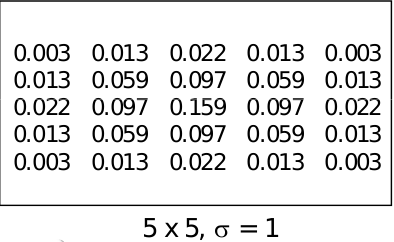
\includegraphics[width=0.75\textwidth]{./imgs/gaussian_kernel.png}
	\caption{\footnotesize Notar los elementos que se repiten y los patrones en la forma localización en que estos se ubican.}
	\label{fig:lineplot.diff}
\end{figure}


Al analizar varios casos de matrices guassianas surgió una regla general facil de implementar la cual utilizamos en esta implementación. Dado un elemento del kernel $k_{i,j}$ nos dimos cuenta que tendra a lo sumo 7 elementos iguales. Entre los 8 tendremos a $k_{i,j}$, $k_{-i,j}$, $k_{i,-j}$, $k_{-i,-j}$, $k_{j,i}$, $k_{-j,i}$, $k_{j,-i}$ y $k_{-j,-i}$. Notar que ocurre si uno de los dos elementos es 0, en ese caso sera indistinto -0 y +0 por lo que se repetiran en estos casos la mitad de elementos de lo normal, lo mismo ocurrira cuando j e i tengan un valor absoluto igual.

Estas particularidades pueden aprovecharse para que al aplicar el filtro y hacer los calculos tomemos de una sola vez todos los pixels que seran multiplicados por elementos iguales del kernel y asi ahorra accesos a memoria y calculos ya que la cantidad de multiplicaciones que hacemos se reduce a la cantidad de elementos distintos en la matriz.

\newpage

\section{Resultados}
\subsection{Estudio sobre la relación entre la representación numérica escogida y los tiempos de ejecución}

\subsubsection{Introducción}

Al analizar nuestra implementación del blur gaussiano en busca de una posible
mejora o variante que pueda resultar de interes surgio la idea de cambiar el
sistema de representación numerica que se utilizaba, la versión base utiliza
double lo cual asegura una buena precisión al hacer los cálculos, pero muchas
veces esta precisión no es necesaria y se prefiere una performance mayor en
terminos de tiempos de ejecución a partir de esto surge la idea de nuestro
experimento.

\subsubsection{Hipotesis del Experimento}

A partir de las ideas mencionadas surge entonces un experimento para intentar
corroborar esta intuición acerca de como al sacrificar precisión podemos quizas
obtener un filtro de mayor velocidad. Creemos que si trabajamos con floats y
necesitamos para ellos 32 bits, entonces, al pasar nuestra implementación a 16
bits utilizando unsigned short podremos acercarnos a una disminución en el
tiempo de ejecución de la mitad. Esta idea se fundamenta a partir de como
gracias a las instrucciones que assembler posee para operar con multiples
paquetes de datos (SIMD) podemos trabajar con el doble de paquetes si son de la
mitad de tamaño que antes. Un punto importante con el que tuvimos que
enfrentarnos fue como adaptar el algoritmo para hacer perder la menor cantidad
de precisión posible. Para esto antes armamos una variante del kernel que en vez
de trabajar con numeros entre 0 y 1 trabajaba con numeros entre 0 y 255, valores
con los que unsigned short puede manejarse bien, una mejor explicación de la
implementación de este algoritmo esta en la sección de Descripción del codigo en
el informe.

\subsubsection{Metodos utilizados}

Para corroborar nuestra hipotesis generamos un conjunto de imagenes cuadradas
con pixels de colores seleccionados de forma aleatoria, para hacer esto creamos
el archivo llamado random\_images\_generayor.py el cual tiene instrucciones de
uso detalladas en sus comentarios, de todas maneras el funcionamiento de nuestro
blur gaussiano no depende del color de los pixels por lo que se podria haber
utilizado cualquier conjunto de imagenes no necesariamente aleatorias. A partir
de esto creamos imagenes de 5 tamaños distintos, que iban de 25x25 hasta
400x400. Luego repitiendo los experimentos de forma suficiente como para
disminuir la varianza al máximo. Una vez obtenidos estos resultados analizamos
que tanto bajo la calidad de la imagen para esto nos guiamos primero de la mera
observación y complementandolo con el análisis que bmpdiff nos brinda.

Para los experimentos utilizamos tres implementaciones distintas de blur hechas
en assembler estas son explicadas con detalle en la sección de descripción del
codigo.

\subsubsection{Verificación: Experimento 1}


\begin{figure}[H]
\centering
    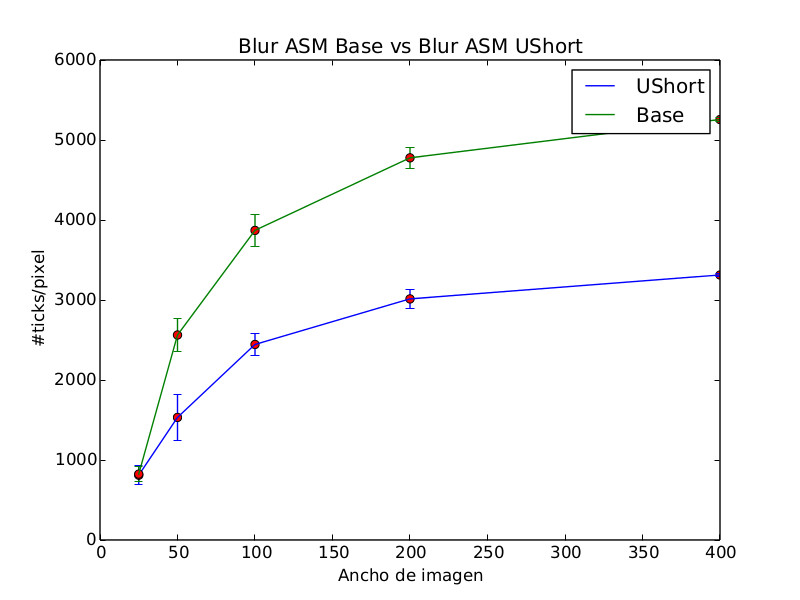
\includegraphics[scale=0.5]{imgs/blur_ushort.jpg}
  \caption{\footnotesize{Grafico donde se observan los tiempo de ejecución de las dos implementaciones estudiadas funcionando con distintos tamaños de imagenes.}}
  \label{fig:tiempo2}
\end{figure}

\begin{figure}[H]
\centering
\begin{minipage}{0.48\textwidth}
  \centering
    
\includegraphics[width=1\textwidth]{imgs/chip_hd_v1.jpg}
  \caption{\footnotesize{Imagen filtrada con blur\_asm\_v1 ($\sigma$ = 3 $r$ = 9), no presenta problemas para mantener el brillo de la imagen.}}
  \label{fig:tiempo1}
\end{minipage}%
\hspace{0.03\textwidth}
\begin{minipage}{0.48\textwidth}
  \centering
    
\includegraphics[width=1\textwidth]{imgs/chip_hd_ushort.jpg}
  \caption{\footnotesize{Imagen filtrada con blur\_asm\_ushort ($\sigma$ = 3 $r$ = 9), la versión que utiliza unsigned short, se nota el oscurecimiento ocasionado probablemente por la perdida de precisión en los cálculos.}}
  \label{fig:tiempo2}
\end{minipage}
\end{figure}


\subsubsection{Verificación: Experimento 2}

Si bien el resultado anterior fue muy prometedor, ya que este mostraba
resultados bastante concluyentes sobre como el tiempo de ejecución habia casi
disminuido a la mitad, de todas maneras notamos que la utilización de unsigned
int en la nueva implementación habia tenido ciertos cambios ajenos al tamaño de
la estructura del dato que podian llegar a contribuir en la velocidad de
computo. La principal sospecha surgió de las instrucciones de conversión de
punto flotante a int (y de int a punto flotante), estas aparecen en
blur\_asm\_v1 pero dejan de ser necesarias en blur\_asm\_ushort.

Para verificar que la influencia de estas instrucciones no era tan grande
implementamos blur\_asm\_uint, esta variante de blur, utiliza unsigned int por
lo que siempre nos mantenemos en representaciones de punto fijo evitando
conversiones. La gran diferencia con la implementación que utiliza shorts es que
el tamaño requerido para hacer los cálculos no va a ser distinto del necesario
en la implementacion base, blur\_asm\_v1.

Los resultados fueron sorpresivos, la influencia de las instrucciones de
conversion parecio casi nula en la velocidad de computa de los programas. Esto
se puede observar en los siguientes gráficos.

\begin{figure}[H]
\centering
    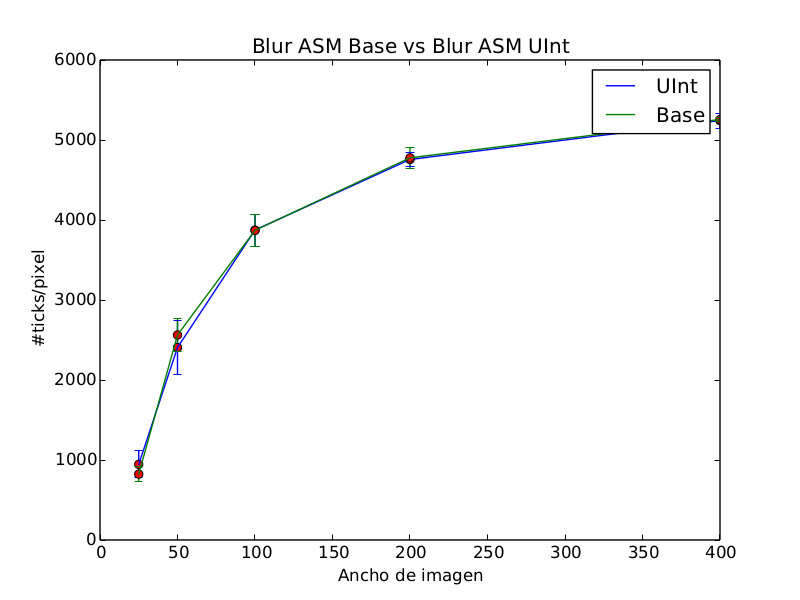
\includegraphics[scale=0.5]{imgs/blur_uint.jpg}
  \caption{\footnotesize{Grafico donde se observan los tiempos de ejecución de las dos implementaciones estudiadas funcionando con distintos tamaños de imagenes.}}
  \label{fig:tiempo1}
\end{figure}

Otro detalle relevante es que observamos como en este caso no se perdia brillo
como pasaba con la implementación de blur UInt, se nota como la mayor cantidad
de bits permiten una precisión suficiente para no redondear tanto los numeros
para abajo y evitando acercarnos a valores cercanos a 0 en la paleta de colores.

\begin{figure}[H]
\centering
    
\includegraphics[scale=0.5]{imgs/chip_hd_uint.jpg}
  \caption{\footnotesize{Imagen filtrada con el blur\_asm\_uint, valores utilizados $\sigma$ = 3 $r$ = 9}}
  \label{fig:tiempo1}
\end{figure}

\newpage

\section{Conclusiones}
Este trabajo nos permitió ver en casos reales las ventajas del procesamiento de
datos en simultáneo. A su vez pudimos comparar qué tanto mejora el realizar una
implementación en ASM contra una en C, logrando así tener una mejor idea de
cuándo realmente conviene decidirse por uno o por el otro.

Por un lado vimos que en lo que era \textit{Diferencia de Imágenes}, la
implementación en ASM superó en forma desmedida la de C incluso con
optimzaciones del compilador. Sin embargo con \textit{Blur Gaussiano} esta
diferencia no fue tan abismal para la implementación de control, e incluso con
la versión en C mejorada para utilizar mejor la matriz de convolución pudimos
observar cómo nuestra versión en ASM se quedaba atrás. Esto refleja cómo algunas
implementaciones en C el compilador es capaz de optimizar mejor que otras,
llevándonos a repensar cómo mejorar nuestros programas.

En lo que respecta la precisión contra el rendimiento en el algoritmo de
\textit{Blur Gaussiano}, los resultados fueron en parte alentadores, porque
vimos cómo se reducía el tiempo de cómputo, pero a su vez nos mostró que a veces
la precisión es un factor que afecta considerablemente el resultado, como lo fue
en nuestro caso.

Por último, quedan muchos experimentos más que se podrían haber realizado así
como profundizado. En particula, con la cuestión de precisión contra
rendimiento, se podrían haber realizado un mayor número de pruebas, variando los
parámetros de entrada para así poder observar con mayor detenimiento si era en
todos los casos que la imagen resultante se veía afectada, o sólo en cierto
rango. A su vez, se podría mejorar el código para que en lugar de trabajar con
unsigned shorts, lo hiciera con unsigned bytes, nuevamente duplicando la
cantidad de pixeles a procesar en simultáneo.

\newpage

\end{document}
